\documentclass[11pt,letterpaper]{article}
\usepackage[margin=1in]{geometry}
\usepackage[T1]{fontenc}
\usepackage{graphicx,amsmath,pdflscape,booktabs,float}
\usepackage{hyperref}
\urlstyle{same}
\hypersetup{colorlinks=true,linkcolor=blue,urlcolor=blue}
\setlength{\parindent}{0pt}
\setlength{\parskip}{0.38em}
\setlength{\emergencystretch}{2em}
\newcommand{\codelink}[2]{\href{https://github.com/RohMalpani/CS422Assignments/blob/main/assignment2/#2}{#1}}
\title{Assignment 2: iPerf, TCP Statistics,\\and Congestion Control}
\author{Annsh Navle, Rohan Malpani, Valmik Vyas}
\date{CS 422 -- Fall 2026}



\begin{document}
\maketitle
\section*{Repository}
The source code, input server list, raw measurements, Dockerfile, and plotting
scripts are available in the
\href{https://github.com/RohMalpani/CS422Assignments/tree/main/assignment2}{Assignment 2 repository folder}.
This report follows Questions 1--3 of the assignment. Parts 1 and 2 use CUBIC;
Part 3 compares CUBIC, Reno, and BBR before proposing a new controller.

To regenerate the figures and tables from the saved measurements, run from
\texttt{assignment2/}:
\begin{verbatim}
python3 run_all.py --replot-only \
  --part3-out-dir results/part3-live \
  --part3-plots-dir plots/part3-live
tectonic report.tex
\end{verbatim}
Dependencies, live-experiment options, and Docker commands appear in Section~\ref{sec:reproduce}.


\section{iPerf Throughput Application}

\subsection{Client implementation and destination selection (Questions 1a--b)}

Our Python client uploads data to standard public iperf3 servers without
invoking the iperf3 binary or using a custom receiver.
\codelink{\texttt{run\_test}}{part1/iperf3_client.py\#L91} opens the control
connection, negotiates JSON test parameters, and opens a data connection with
the same session cookie. After the server starts the test,
\codelink{\texttt{\_send\_data}}{part1/iperf3_client.py\#L162} sends continuously
for the configured duration. The client sends \texttt{TEST\_END}, exchanges
results, and terminates with \texttt{IPERF\_DONE}. Five-second connection and
ten-second I/O timeouts bound non-response. Rejections, unexpected states,
closed connections, and socket errors are logged as failed attempts.


\codelink{\texttt{ServerPool}}{part1/select_servers.py\#L44} randomly shuffles
entries from \texttt{servers.csv}, sourced from iperf3serverlist.net, and selects
entries without replacement, choosing a random port from each advertised range.
The driver replaces failed destinations until the requested count is reached,
the list is exhausted, or ten attempts have failed.

The October 17 experiment contains ten successful destinations, one
60-second transfer per destination, and a nominal one-second sampling interval.
All successful data sockets reported CUBIC via \texttt{TCP\_CONGESTION}.
There were two failed attempts: Vienna (\texttt{185.180.12.40:5201}) returned
\texttt{ACCESS\_DENIED}, and Pune (\texttt{69.48.236.198:30004}) returned a
broken-pipe error. Both were replaced; there was no destination shortfall.
Selected addresses, ports, and attempt outcomes are recorded in
\codelink{\texttt{part1\_runs.csv}}{results/part1_runs.csv}.
The project log records WSL2, Ubuntu 22.04, Python 3.10, and kernel series 6.6;
the exact kernel release was not saved.

\subsection{Acknowledged goodput (Question 1c)}

\codelink{\texttt{GoodputSampler}}{part1/goodput.py\#L47} reads cumulative
\texttt{tcpi\_bytes\_acked} through \texttt{getsockopt(TCP\_INFO)} on the
\emph{data socket}. For acknowledged bytes $A_i$ and actual elapsed time $t_i$,
\[
G_i=\frac{8(A_i-A_{i-1})}{t_i-t_{i-1}}\;\text{bits/s}.
\]
Using acknowledged bytes avoids counting data only buffered by \texttt{send()}.
Actual sampling intervals, rather than the nominal one second, are used.
The initial counter is zero, so the first interval can include a small protocol
byte offset. Raw samples are saved in
\codelink{\texttt{part1\_samples.csv}}{results/part1_samples.csv}.


\subsection{Results and discussion}

\begin{table}[H]
\centering
\small
\begin{tabular}{lrrrr}
\toprule
Destination & Min & Median & Mean & P95 \\
\midrule
Algiers & 2.53 & 177.12 & 154.12 & 179.28 \\
Alvsjo & 1.46 & 136.51 & 108.54 & 140.50 \\
Helsinki & 1.58 & 158.46 & 134.46 & 181.32 \\
Istanbul & 1.33 & 153.80 & 123.70 & 155.75 \\
London & 7.09 & 20.86 & 26.83 & 62.53 \\
Montreal & 303.85 & 453.87 & 451.07 & 461.82 \\
Paris & 1.06 & 69.45 & 61.85 & 110.17 \\
Phoenix & 225.01 & 378.25 & 376.04 & 392.22 \\
Plano & 293.76 & 436.40 & 440.43 & 472.52 \\
Reykjavik & 12.85 & 167.07 & 164.46 & 170.12 \\
\bottomrule
\end{tabular}
\caption{Goodput in Mbps for CUBIC. Each destination has 60 interval samples.
Statistics include startup; the mean weights samples equally, and P95 uses
linear interpolation. Generated by
\codelink{\texttt{summary\_table}}{part1/plot_goodput.py\#L75}.}
\label{tab:part1-summary}
\end{table}

Table~\ref{tab:part1-summary} and Figure~\ref{fig:part1-goodput} summarize
the ten destinations. Montreal achieved the highest mean goodput (451.07 Mbps), followed by Plano
(440.43 Mbps) and Phoenix (376.04 Mbps). London had the lowest mean
(26.83 Mbps). These results describe the observed paths during the experiment,
not the servers' maximum capacities.

Algiers and Istanbul ramped up before stabilizing near 179 and 154 Mbps,
respectively. Paris reached approximately 108 Mbps only after about 34 seconds,
which reduced its full-run mean to 61.85 Mbps. This startup behavior is
consistent with TCP increasing its sending window. London showed an early
spike followed by a substantial decline, while Helsinki had intermittent drops.
Goodput alone cannot distinguish congestion, loss recovery, and receiver limits.
With only one run per destination, these results do not establish repeatability.

\begin{figure}[H]
\centering
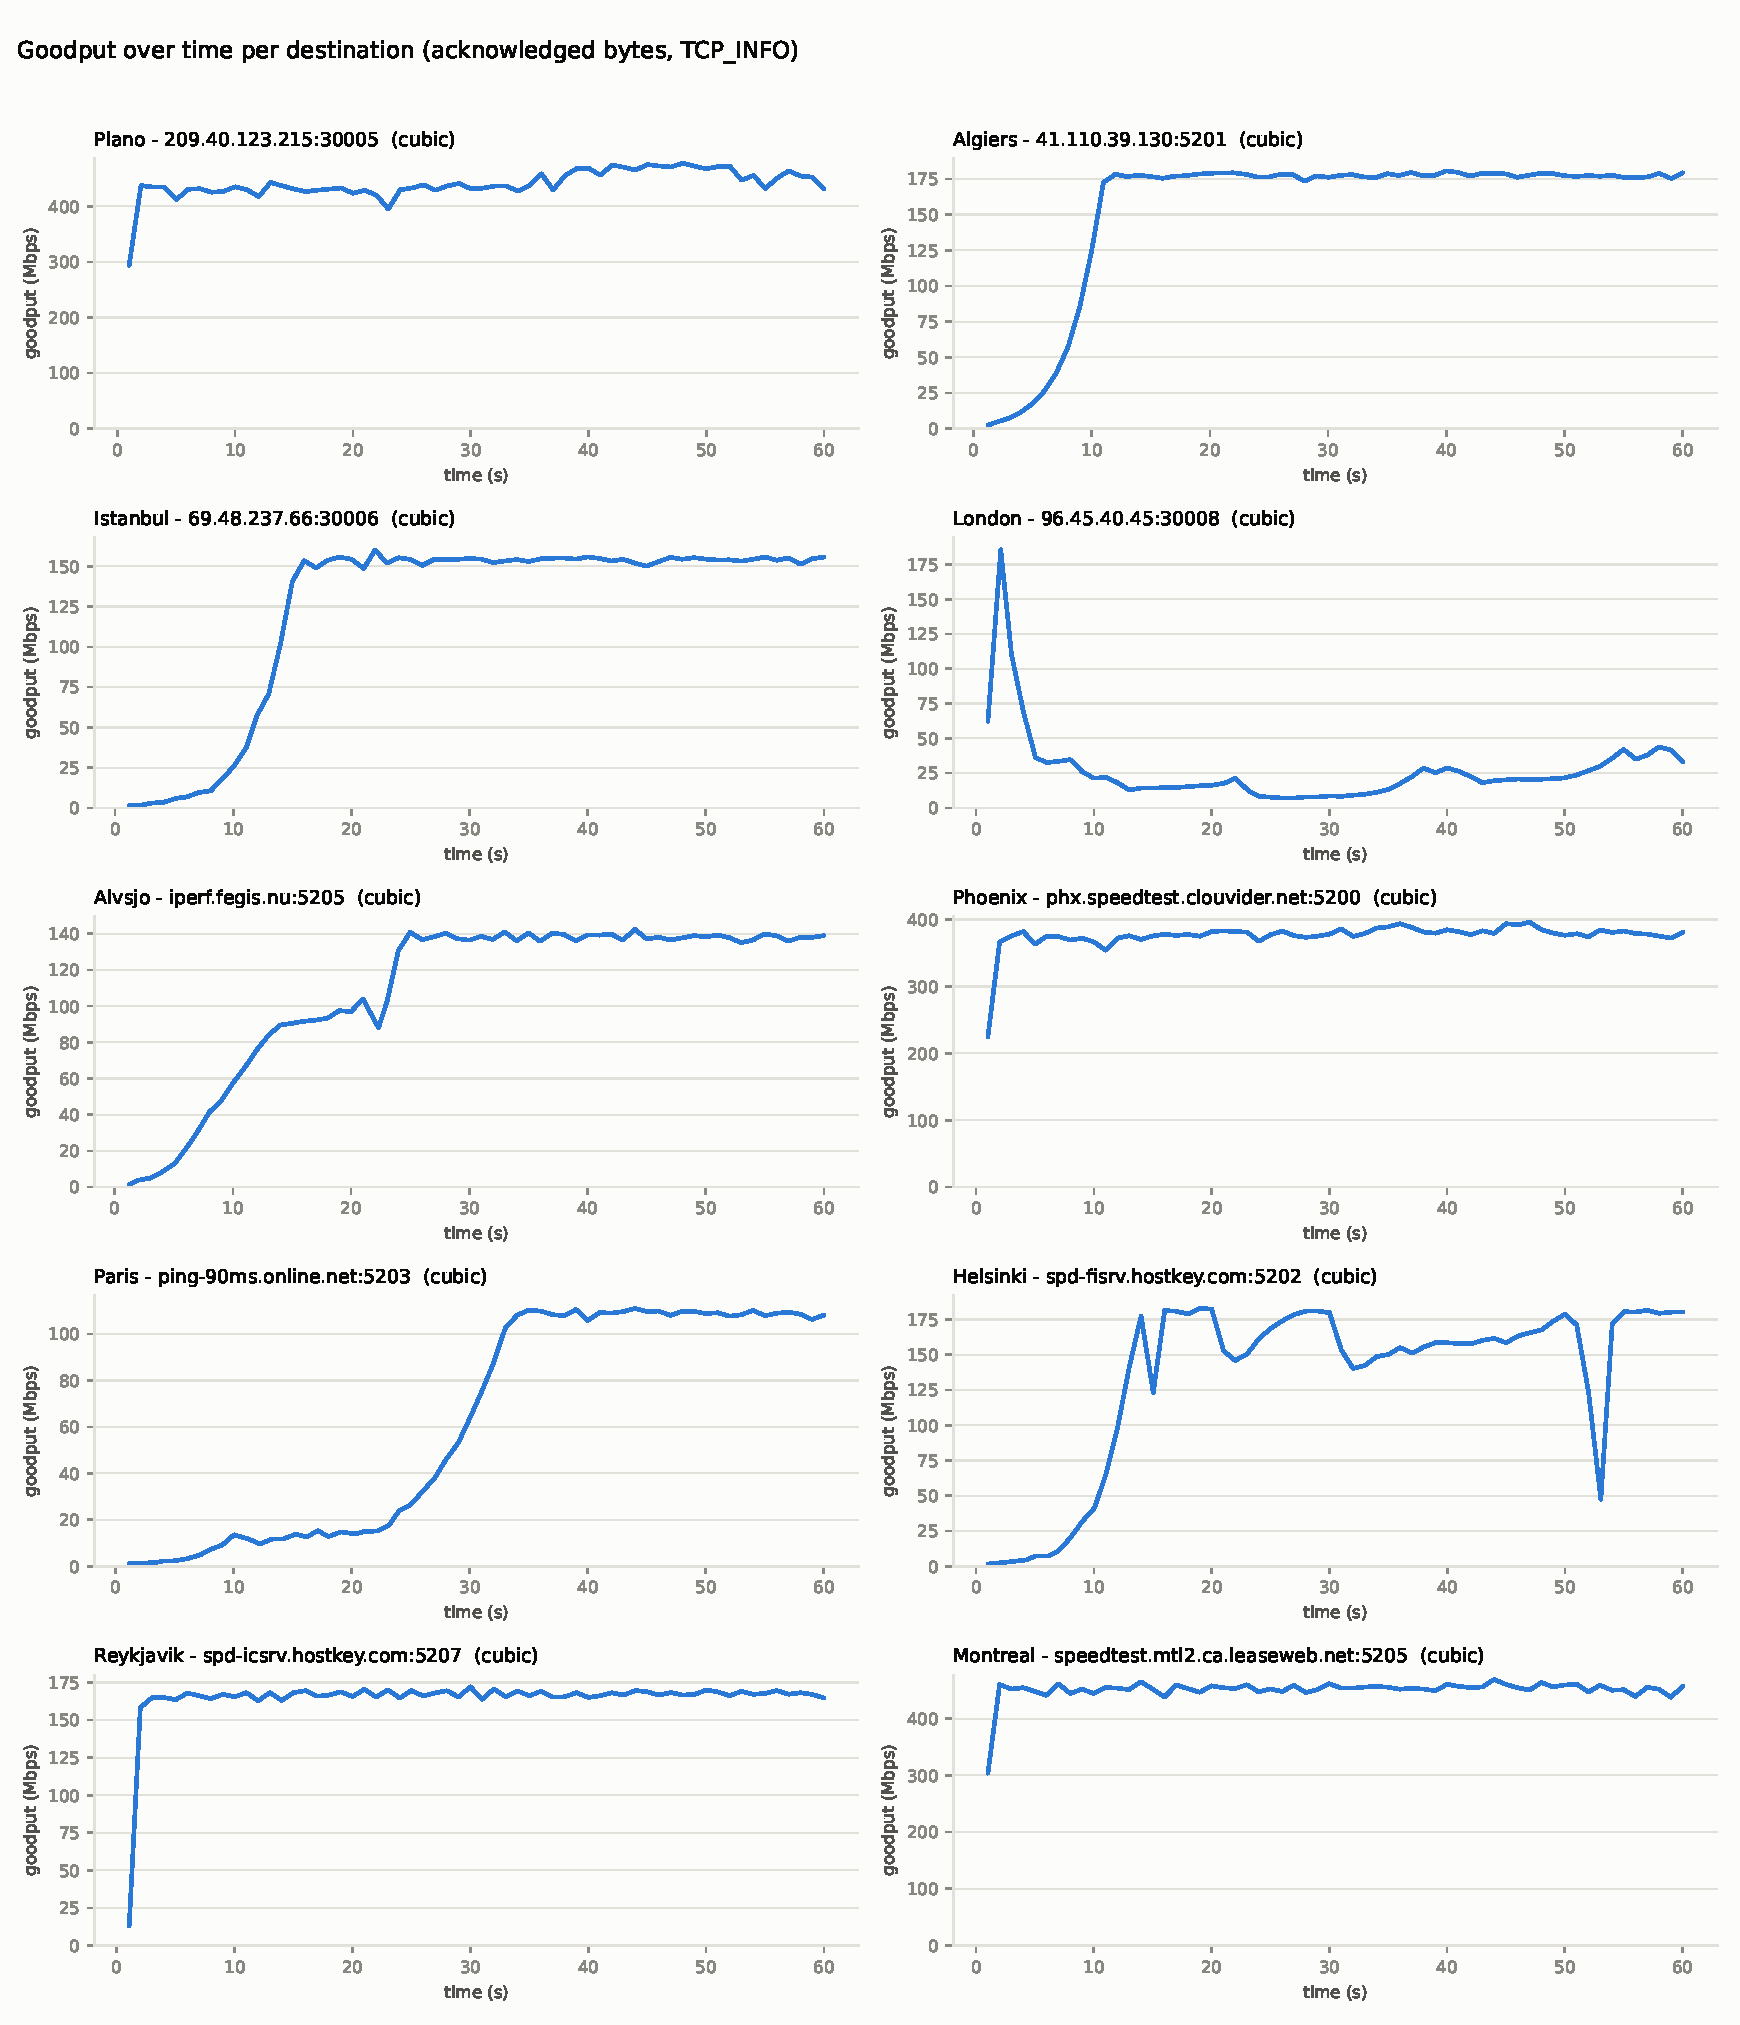
\includegraphics[width=\textwidth,height=0.65\textheight,keepaspectratio]{plots/part1_goodput.pdf}
\caption{Goodput over time for all ten destinations, generated by
\codelink{\texttt{plot\_goodput}}{part1/plot_goodput.py\#L25}.
Each panel uses its own vertical scale and labels the server address, port,
and actual algorithm.}
\label{fig:part1-goodput}
\end{figure}


\clearpage\section{TCP Statistics During Transfer}

\subsection{Method and decoding format (Question 2a)}

Part 2 reuses the live data-socket measurements collected in Part 1. The
representative destination is Algiers (\texttt{41.110.39.130:5201}), selected
by the plotting script as the destination whose mean goodput is closest to the
median of the destination means. This trace contains 60 samples from one
60-second run; the recorded algorithm is CUBIC.

\codelink{\texttt{read\_tcp\_info}}{part1/goodput.py\#L32} requests 256 bytes
using \texttt{getsockopt(TCP\_INFO)}. An ordered field table mirrors Linux's
\texttt{struct tcp\_info}, using native byte order and fixed-width unsigned
8-, 32-, and 64-bit fields; decoding stops at the returned buffer length.
The project log records validation against C field offsets on WSL2.

Each CSV sample records a timestamp, elapsed interval, congestion window
(\texttt{snd\_cwnd}, segments), smoothed RTT (\texttt{rtt\_us}, microseconds),
and goodput (bits/s). It also includes RTT variation, acknowledged bytes,
pacing and delivery rates, destination, run identifier, repetition, and actual
algorithm. The loss proxy is
\[
L_i=\mathrm{total\_retrans}_i-\mathrm{total\_retrans}_{i-1}.
\]
This counts retransmitted segments during an interval, not a packet-loss
percentage; retransmissions can also be spurious. Goodput uses the actual
elapsed interval as described in Part 1.

\subsection{Visualizations and observations (Questions 2b--c)}
The following seven plots use the same Algiers CUBIC trace. The code that
produces them is
\codelink{\texttt{plot\_tcp\_stats}}{part2/plot_tcp_stats.py\#L72}.

\clearpage
\subsubsection{Congestion window and acknowledged goodput}
\begin{center}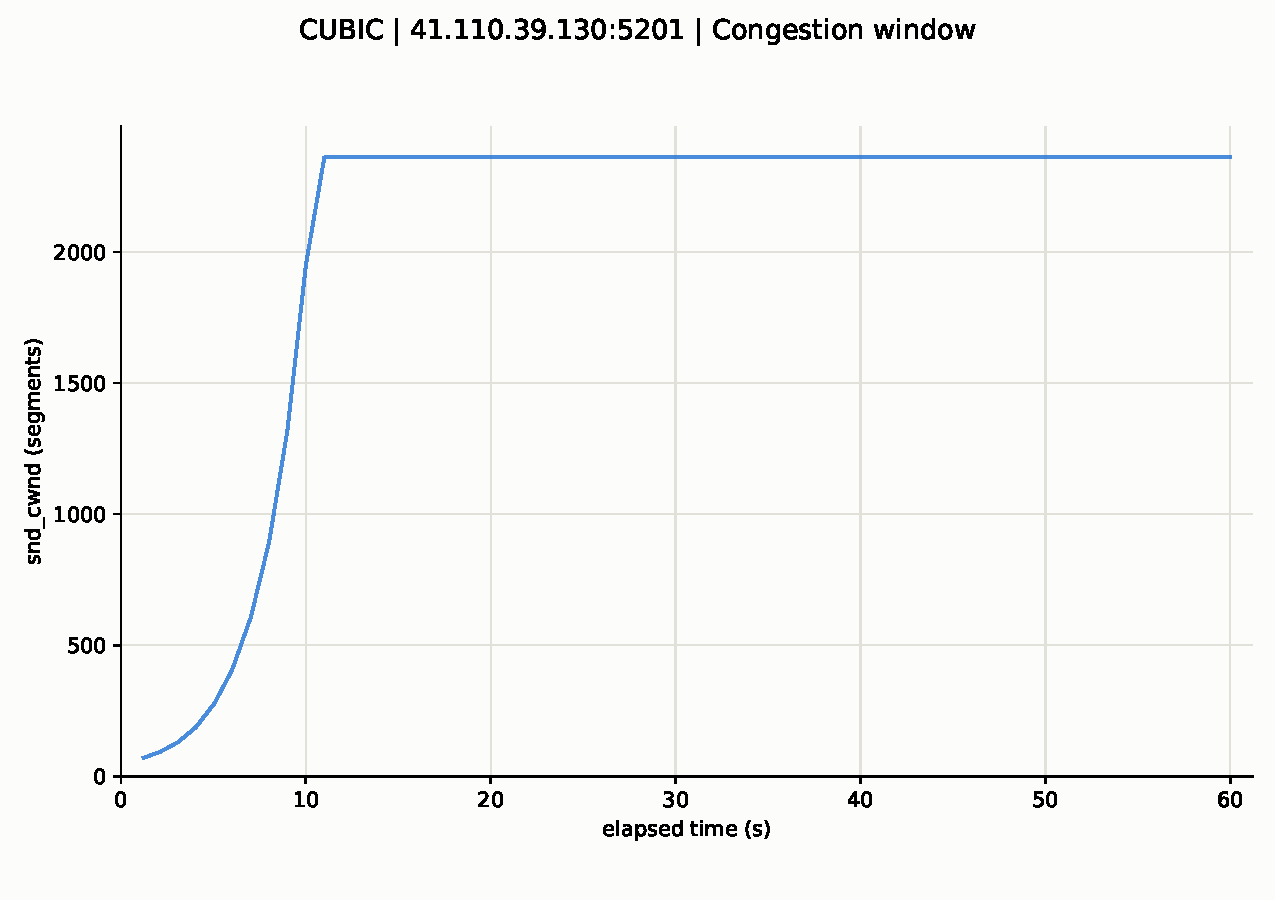
\includegraphics[page=1,width=0.70\textwidth]{plots/part2_tcp_stats.pdf}\end{center}
\begin{center}\includegraphics[page=4,width=0.70\textwidth]{plots/part2_tcp_stats.pdf}\end{center}
The congestion window is the maximum number of segments TCP allows in flight.
During congestion avoidance, a larger window can raise goodput when the flow
is window-limited; it cannot increase capacity once the bottleneck is full.
Here the window grows from 70 to 2,361 segments by 11 seconds, while goodput
rises from 2.53 to 172.41 Mbps. The window then stays fixed and goodput
settles near 177--179 Mbps. The early ramp includes startup, so it is not
pure congestion-avoidance behavior.

\clearpage
\subsubsection{RTT and the loss proxy}
\begin{center}\includegraphics[page=2,width=0.70\textwidth]{plots/part2_tcp_stats.pdf}\end{center}
\begin{center}\includegraphics[page=3,width=0.70\textwidth]{plots/part2_tcp_stats.pdf}\end{center}
RTT is the kernel's smoothed estimate of a data/ACK round trip. For a fixed
window, a larger RTT reduces the window-limited rate; rising RTT can also
indicate queueing. RTT starts at 195.15 ms and falls to about 122 ms by the
third sample, an unusual transient whose cause is not identified by this trace.
The loss signal counts new retransmitted segments per interval. Loss recovery
can reduce the window and goodput, but all intervals here have zero
retransmissions, so this run provides no observed loss response.

\clearpage
\subsubsection{Window and RTT relationships with goodput}
\begin{center}\includegraphics[page=5,width=0.70\textwidth]{plots/part2_tcp_stats.pdf}\end{center}
\begin{center}\includegraphics[page=6,width=0.70\textwidth]{plots/part2_tcp_stats.pdf}\end{center}
Each point pairs a socket measurement with the goodput of its sampling
interval. The window scatter shows the startup rise and the later plateau.
The RTT scatter mixes the early RTT transient with steady operation; it does
not show that changing RTT caused the goodput change. In the window-limited
case, the expected rate is approximately window bytes divided by RTT, while
path capacity, pacing, and the receiver window can impose other limits.

\clearpage
\subsubsection{Loss relationship with goodput}
\begin{center}\includegraphics[page=7,width=0.70\textwidth]{plots/part2_tcp_stats.pdf}\end{center}
Every point lies at zero retransmissions despite a wide range of goodput.
The absence of retransmissions therefore does not imply that maximum goodput
has already been reached. This run cannot establish the effect of loss on
goodput, and a single repetition cannot establish repeatability.


\clearpage\section{Algorithm Comparison and Controller Design}

\subsection{Experiment method (Question 3a)}

The October 22 experiment tests CUBIC, Reno, and BBR
on ten selected destinations for three scheduled repetitions, 60 seconds per
test, and a nominal one-second sampling interval. The experiment ran on an
Ubuntu 24.04 Multipass VM with kernel \texttt{6.8.0-147-generic}. The environment
record lists all three algorithms as available and allowed, with CUBIC the
default; these kernel settings were checked after the run, not at launch.

\codelink{\texttt{collect\_one}}{part3/compare_algorithms.py\#L65}
selects the algorithm on the data socket before connecting and verifies the
actual value. All successful selected-path tests match the requested algorithm.
The order rotates through CUBIC--Reno--BBR, Reno--BBR--CUBIC, and
BBR--CUBIC--Reno according to destination index and repetition. For Floreal,
these are the orders in repetitions 1, 2, and 3, respectively. Exact order is
stored in \texttt{test\_order}; tests are sequential with a one-second cooldown.

There were 108 attempts: 88 successes and 20 failures. Six candidate destinations
were replaced during selection; three successes on these rejected candidates
are excluded from comparison. All ten requested destinations were selected.
The selected set has 85 successful tests (5,100 samples); in repetition 3,
CUBIC and BBR tests failed for Tallinn, and all three failed for San Jose. Failed/partial
runs remain in the raw logs but do not contribute to statistics.

Table~\ref{tab:matched} uses only destination--repetition combinations
where all three algorithms succeeded: 28 matched triples (84 tests).
Tallinn and San Jose therefore contribute two matched repetitions; other sites
contribute three. Table~\ref{tab:part3-summary} includes all
85 successes, including Tallinn's unmatched third Reno run.


\subsection{Matched results}

\begin{table}[H]
\centering
\small
\begin{tabular}{lrrrrrr}
\hline
& \multicolumn{3}{c}{Goodput (Mbps)} & \multicolumn{3}{c}{RTT (ms)} \\
Destination & CUBIC & Reno & BBR & CUBIC & Reno & BBR \\
\hline
Amsterdam & 135.40 & 121.12 & 139.90 & 140.03 & 143.55 & 149.38 \\
Dallas & 266.25 & 242.49 & 277.82 & 87.72 & 83.73 & 89.30 \\
Floreal & 46.97 & 62.41 & 57.35 & 346.87 & 339.60 & 338.76 \\
Kyiv & 88.46 & 119.92 & 103.40 & 177.62 & 184.57 & 190.10 \\
Maidenhead & 115.52 & 111.14 & 110.26 & 154.82 & 155.49 & 172.35 \\
Norderstedt & 130.63 & 150.89 & 132.88 & 146.24 & 145.34 & 149.55 \\
Portmore & 101.98 & 70.05 & 183.02 & 98.79 & 99.84 & 116.97 \\
San Jose & 234.34 & 254.41 & 239.28 & 92.59 & 92.33 & 97.40 \\
Sao Paulo & 93.31 & 119.55 & 71.33 & 173.77 & 174.61 & 181.18 \\
Tallinn & 96.63 & 61.26 & 104.56 & 178.88 & 189.49 & 186.77 \\
\hline
\end{tabular}

\caption{Means over matched repetitions. Goodput is the arithmetic mean of
interval goodput; RTT is the mean sampled RTT. Each successful test has 60
samples. Generated by \codelink{\texttt{summarize\_results.py}}{part3/summarize_results.py\#L37}.}
\label{tab:matched}
\end{table}

The common representative destination is Floreal,
\texttt{speedtestfl.telecom.mu:5205}, the first selected destination. Figures~\ref{fig:part3-timeseries} and~\ref{fig:part3-scatter} repeat all
seven Part 2 visualizations with identical axis limits across algorithms. Colors identify repetitions.
The \codelink{run log}{results/part3-live/part3_runs.csv} records attempts,
addresses, ports, actual algorithms, and outcomes; the
\codelink{environment record}{results/part3-live/run_environment.txt}
describes the measurement host.


\clearpage

\subsection{Operating regimes and discussion}

\textbf{Long-RTT paths with little recorded loss.}
On Floreal, Reno averages 62.41 Mbps, BBR 57.35 Mbps, and CUBIC 46.97 Mbps.
Reno has only one retransmission across its three runs; it sustains a larger
mean window than CUBIC (3,854 versus 1,745 segments). CUBIC's first ten seconds
average only 3.62 and 3.40 Mbps in runs 1 and 3, whereas late-run rates approach
58--60 Mbps. Startup therefore materially lowers its 60-second mean. This
supports Reno for these particular finite-duration, low-loss observations,
not a general claim that Reno is faster on long-RTT paths.

\textbf{A path with frequent retransmissions.}
On Portmore, BBR averages 183.02 Mbps versus 101.98 for CUBIC and 70.05 for Reno.
BBR also has more retransmissions (2,178 per run on average, versus 1,303 and
575), a larger mean window (4,917 versus 874 and 821 segments), and higher mean
RTT (116.97 versus 98.79 and 99.84 ms). Its delivery-rate-based control sustains
more throughput in this trace, while loss-based window reductions are a
plausible contributor to the lower CUBIC/Reno rates. The higher RTT is
consistent with more queueing, but the observations do not prove that the
algorithm caused the delay or that retransmissions equal congestion loss.

\textbf{Throughput--delay tradeoffs.}
CUBIC leads on Maidenhead at 115.52 Mbps, compared with Reno's 111.14 and BBR's
110.26; its mean RTT is also lower than BBR's (154.82 versus 172.35 ms).
BBR leads on Dallas at 277.82 Mbps, but Reno has lower mean RTT (83.73 versus
89.30 ms). Across matched destination means, Reno leads in goodput on five
paths, BBR on four, and CUBIC on one. BBR does not consistently minimize RTT.

\textbf{Window, RTT, and bandwidth--delay product.}
A window-limited flow has approximate rate $W/\mathrm{RTT}$, with $W$ in bytes.
Keeping a bottleneck busy requires enough in-flight data to cover its
bandwidth--delay product, $B\,\mathrm{RTT}_{\min}$. As an illustrative estimate,
Floreal's Reno mean rate of 62.41 Mbps and minimum sampled RTT of 304.30 ms give
about 2.37 MB in flight. This uses measured goodput as a bandwidth proxy, not
an independently measured link capacity. Segment size was not saved, so the
window in segments cannot be converted exactly to bytes. BBR's larger window
does not alone imply higher goodput because pacing, path capacity, and receiver
limits also matter.

\textbf{Representative plots.}
Floreal's CUBIC run 2 records 84 retransmissions, with window reductions around
29--32 seconds; its goodput falls during recovery. Reno's window and goodput
are steadier after startup. BBR's third run records 40 retransmissions, with
window dips around 19 and 24 seconds. The scatter plots show that a single
window or RTT value can accompany different goodput values across time/runs:
instantaneous window and RTT are compared with goodput averaged over an interval.
These associations do not establish causality.

\textbf{Variability and anomalous runs.}
Amsterdam's Reno run means are 157.00, 60.96, and 145.39 Mbps; the low run has
438 retransmissions. Sao Paulo's BBR means are 109.95, 2.09, and 101.95 Mbps,
with no recorded retransmissions. The latter slowdown cannot be explained by
the loss proxy alone. Both runs are included in the analysis. Public-path load, routing, server limits, and temporal order can
change between tests. Rotation reduces ordering bias but does not remove it;
three repetitions and incomplete final tests do not establish universal winners.
Parts 1/2 and Part 3 used different hosts and destination sets, so their means
are not treated as controlled before/after comparisons.


\clearpage

\clearpage\subsection{Throughput summary for every algorithm}

\begin{table}[H]
\centering
\small
\begin{tabular}{llrrrrr}
\hline
Destination & Algorithm & Runs & Min & Median & Mean & P95 \\
\hline
Amsterdam & BBR & 3 & 3.19 & 143.46 & 139.90 & 165.94 \\
Amsterdam & CUBIC & 3 & 3.02 & 152.80 & 135.40 & 173.40 \\
Amsterdam & RENO & 3 & 13.72 & 149.55 & 121.12 & 170.01 \\
Dallas & BBR & 3 & 28.97 & 283.59 & 277.82 & 362.45 \\
Dallas & CUBIC & 3 & 8.50 & 279.32 & 266.25 & 359.98 \\
Dallas & RENO & 3 & 73.34 & 247.11 & 242.49 & 355.64 \\
Floreal & BBR & 3 & 0.27 & 62.55 & 57.35 & 69.98 \\
Floreal & CUBIC & 3 & 0.68 & 55.24 & 46.97 & 68.72 \\
Floreal & RENO & 3 & 1.08 & 64.85 & 62.41 & 73.34 \\
Kyiv & BBR & 3 & 1.25 & 108.83 & 103.40 & 126.54 \\
Kyiv & CUBIC & 3 & 1.85 & 105.18 & 88.46 & 129.06 \\
Kyiv & RENO & 3 & 2.99 & 123.55 & 119.92 & 139.36 \\
Maidenhead & BBR & 3 & 2.16 & 117.33 & 110.26 & 139.53 \\
Maidenhead & CUBIC & 3 & 4.55 & 122.12 & 115.52 & 170.02 \\
Maidenhead & RENO & 3 & 3.86 & 124.30 & 111.14 & 168.85 \\
Norderstedt & BBR & 3 & 2.60 & 138.64 & 132.88 & 159.43 \\
Norderstedt & CUBIC & 3 & 2.18 & 148.18 & 130.63 & 166.72 \\
Norderstedt & RENO & 3 & 7.91 & 154.08 & 150.89 & 170.71 \\
Portmore & BBR & 3 & 4.34 & 186.42 & 183.02 & 235.86 \\
Portmore & CUBIC & 3 & 8.19 & 73.11 & 101.98 & 236.34 \\
Portmore & RENO & 3 & 17.25 & 52.08 & 70.05 & 198.86 \\
San Jose & BBR & 2 & 18.03 & 248.64 & 239.28 & 273.17 \\
San Jose & CUBIC & 2 & 8.02 & 250.62 & 234.34 & 271.54 \\
San Jose & RENO & 2 & 46.72 & 259.16 & 254.41 & 279.21 \\
Sao Paulo & BBR & 3 & 0.96 & 102.96 & 71.33 & 126.31 \\
Sao Paulo & CUBIC & 3 & 2.04 & 116.36 & 93.31 & 137.00 \\
Sao Paulo & RENO & 3 & 1.74 & 124.27 & 119.55 & 139.14 \\
Tallinn & BBR & 2 & 1.51 & 110.47 & 104.56 & 127.54 \\
Tallinn & CUBIC & 2 & 1.80 & 115.07 & 96.63 & 135.08 \\
Tallinn & RENO & 3 & 2.71 & 92.66 & 75.39 & 132.75 \\
\hline
\end{tabular}

\caption{Part 3 interval goodput in Mbps, pooling successful tests on each
selected destination. Each run has 60 samples; startup is included and P95 is
linearly interpolated. Failed tests are excluded, with the run count reported.}
\label{tab:part3-summary}
\end{table}
Figure~\ref{fig:part3-all} shows every successful selected-path trace.
Per-run goodput, RTT, window, and retransmission statistics are also available in
\path{results/part3-live/part3_per_run.csv}. Both tables and the compact
comparison figures are generated by
\codelink{\texttt{write\_tables}}{part3/summarize_results.py\#L37} and
\codelink{\texttt{compact\_plots}}{part3/summarize_results.py\#L80}.


\clearpage

\clearpage\subsection{Comparison plots (Question 3a)}

\begin{figure}[!ht]
\centering
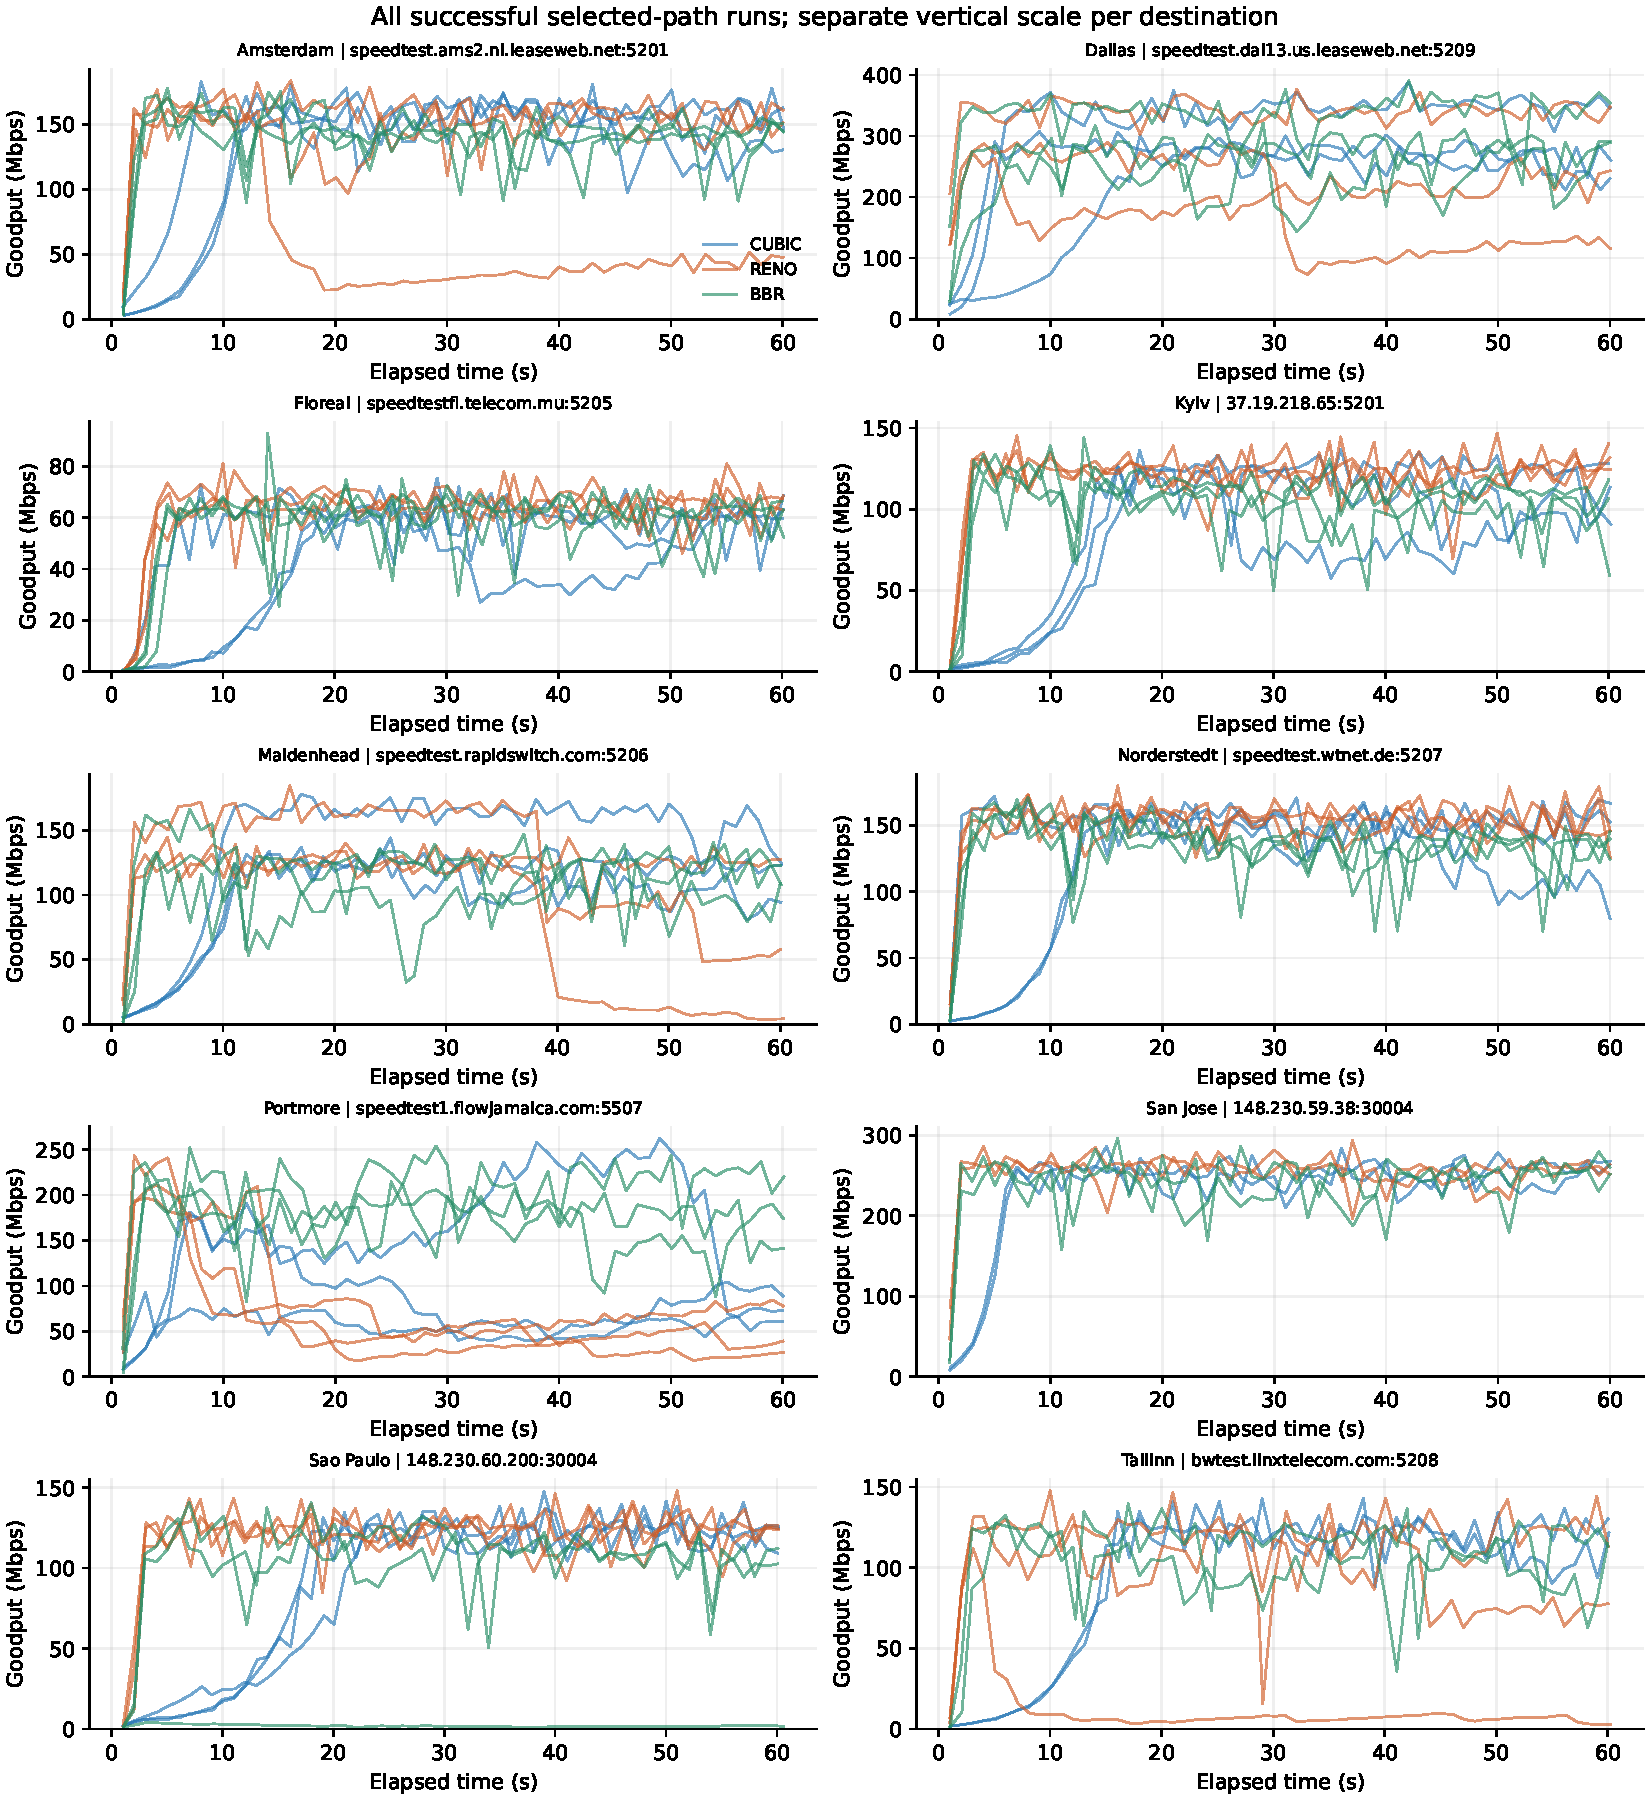
\includegraphics[width=\textwidth,height=0.85\textheight,keepaspectratio]{plots/part3-live/part3_all_goodput.pdf}
\caption{Part 3 goodput for all selected destinations. Each color is an algorithm;
individual repetitions use separate lines. Vertical scales differ by destination.
Only successful tests are shown.}
\label{fig:part3-all}
\end{figure}

\begin{landscape}
\begin{figure}[p]
\centering
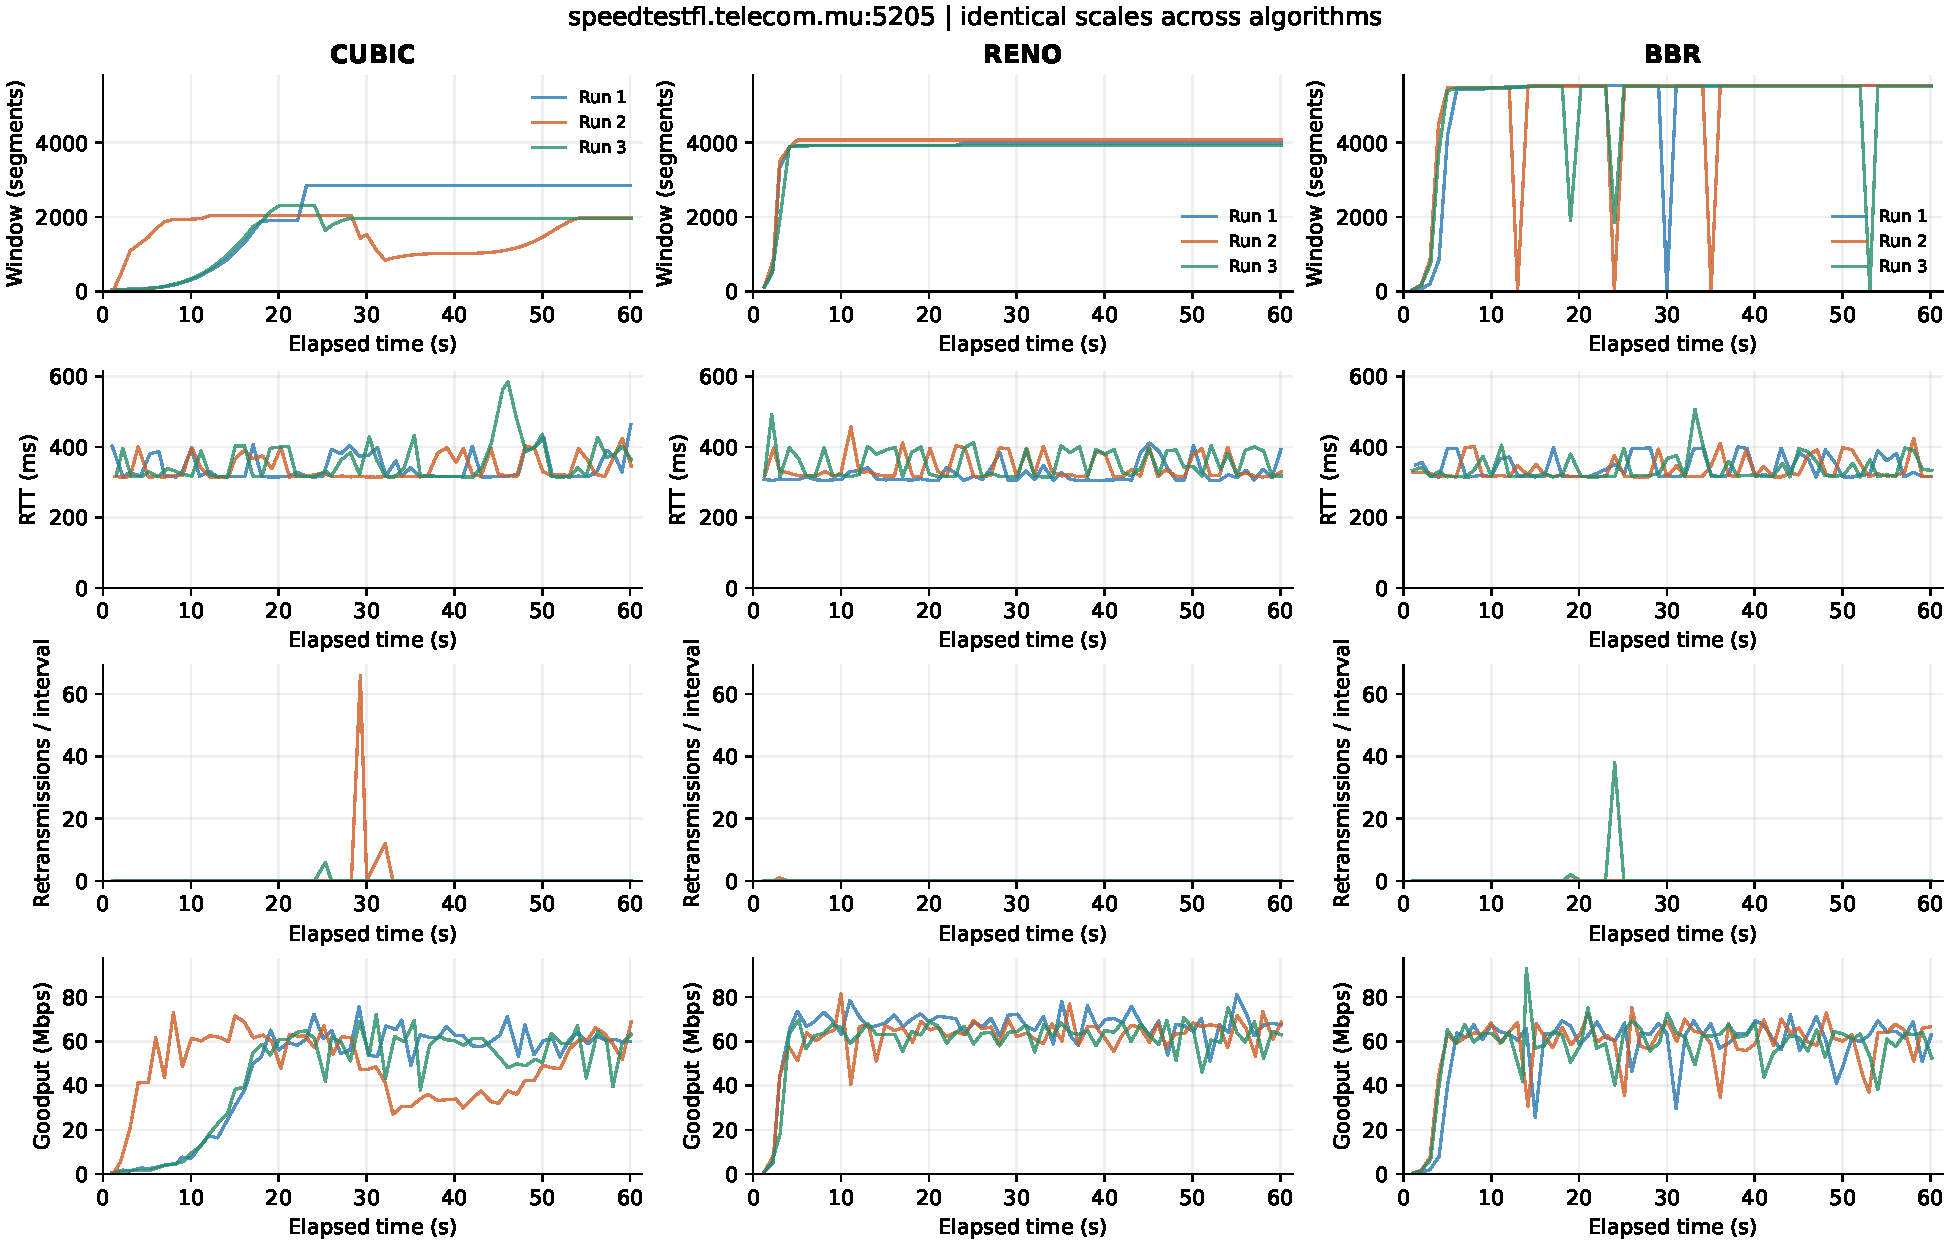
\includegraphics[width=\linewidth,height=0.88\textheight,keepaspectratio]{plots/part3-live/part3_timeseries.pdf}
\caption{Floreal: window, RTT, retransmissions, and goodput for CUBIC, Reno, and BBR.
All three repetitions are shown; corresponding axes use the same limits.}
\label{fig:part3-timeseries}
\end{figure}
\clearpage
\begin{figure}[p]
\centering
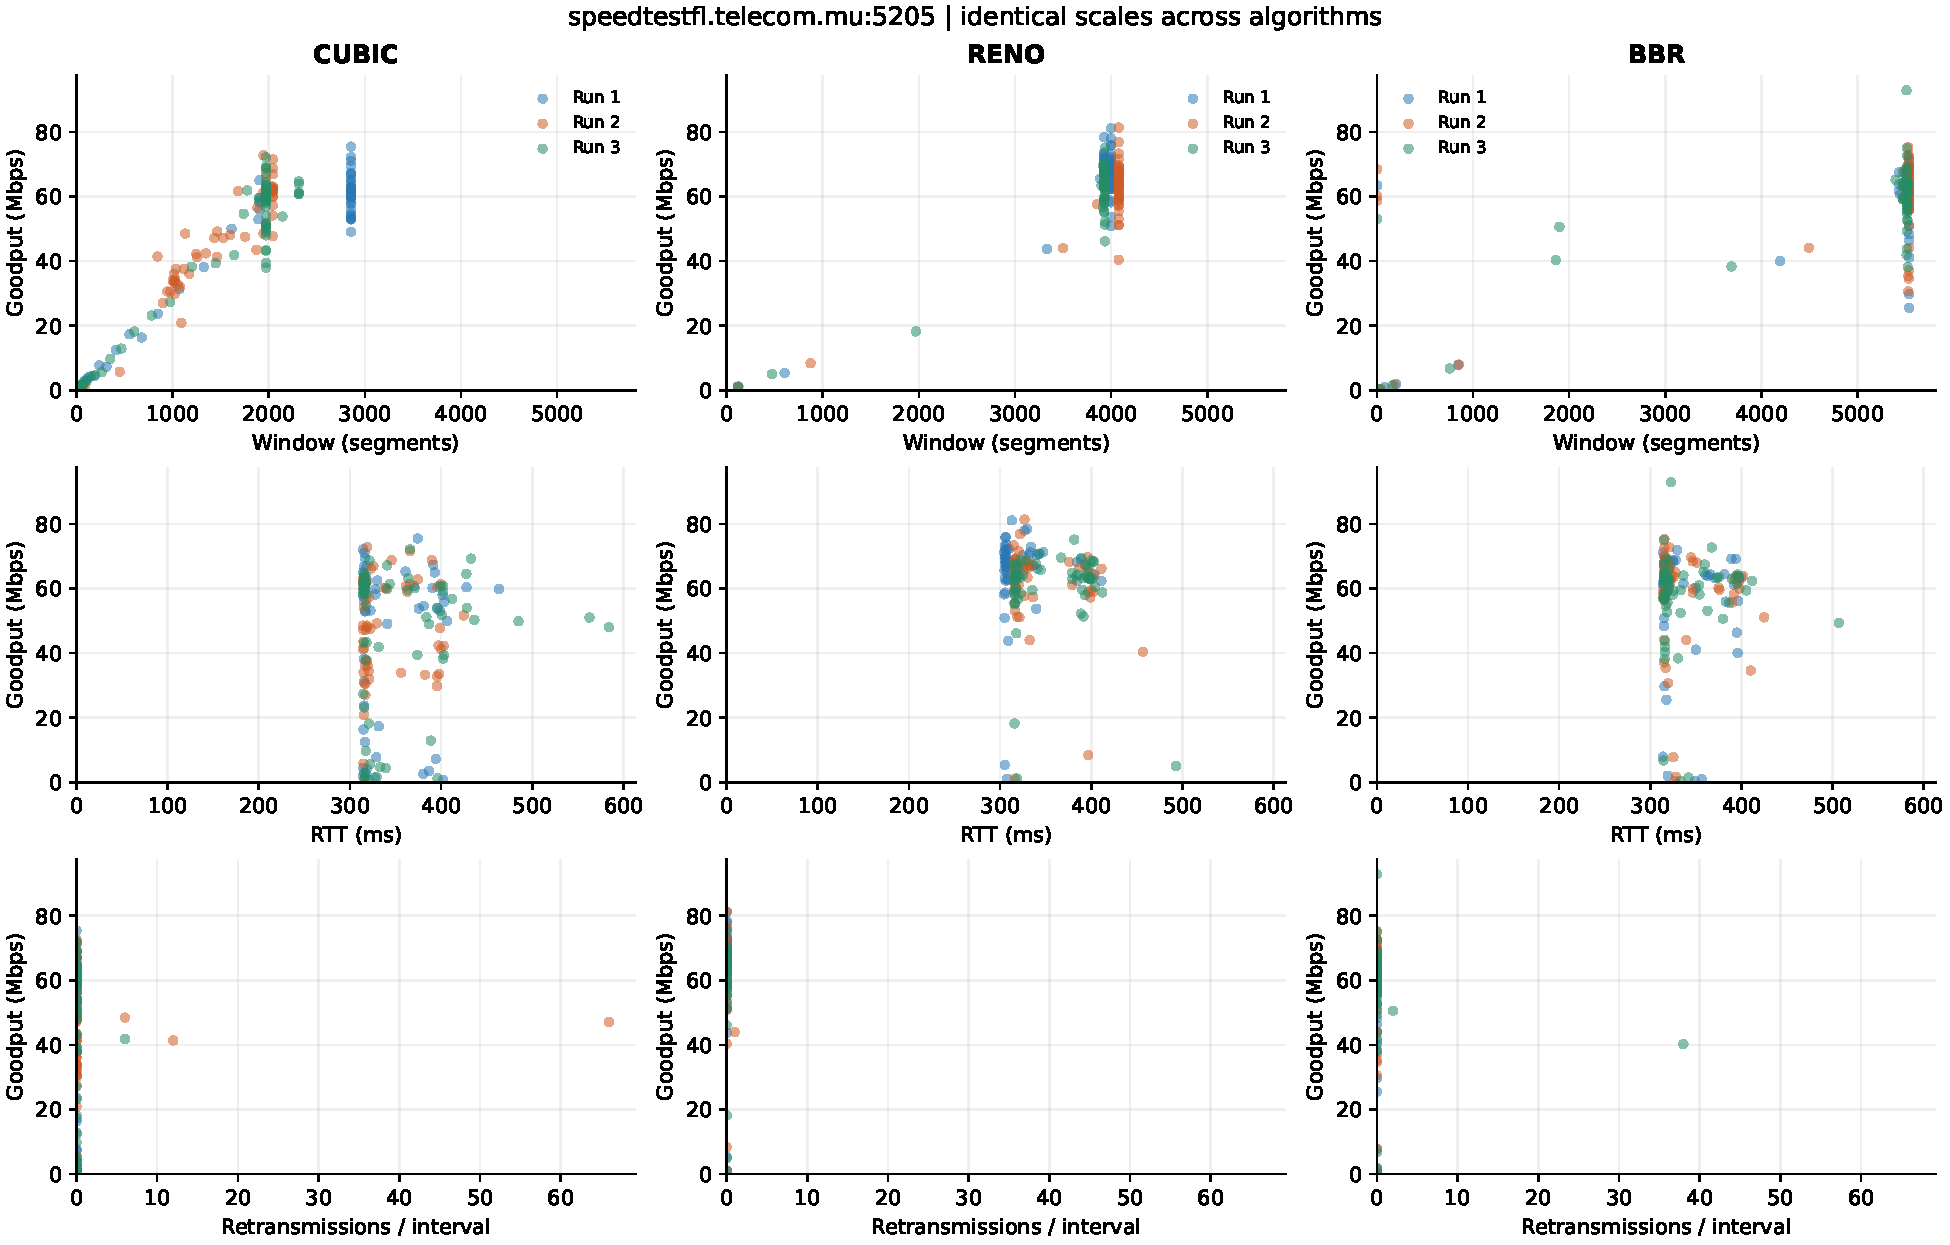
\includegraphics[width=\linewidth,height=0.88\textheight,keepaspectratio]{plots/part3-live/part3_scatter.pdf}
\caption{Floreal: window, RTT, and retransmissions versus goodput for each algorithm.
These are the same samples and repetition colors as the time-series panels.}
\label{fig:part3-scatter}
\end{figure}
\end{landscape}


\clearpage

\subsection{Proposed congestion control algorithm (Question 3b)}

We propose Adaptive Delay/Loss AIMD, a congestion control algorithm that
combines RTT, an ACK-derived delivery-rate estimate, and TCP loss signals to
adjust the congestion window. The pseudocode below specifies the suggested
measurement updates, growth rules, and recovery safeguards. The experiments
in this report evaluate CUBIC, Reno, and BBR; they motivate the proposal but
do not measure the proposed algorithm's performance.

The baseline results motivate Reno-like growth on stable paths, a mild loss
response when delay and delivery remain stable, and early reduction when extra
sending increases delay without improving delivery. These are design hypotheses,
not evidence that the controller improves every path. Its parameters were not
fitted to maximize the reported baseline performance.

\subsubsection{State and measurement updates}
The congestion window $c$ and threshold $s$ are in segments and retain Linux's
initial values. Private state starts at zero, except that the delay-reduction
flag is armed and round time/delivered counters start at their current values.
The smoothed RTT is $r=\texttt{srtt\_us}/8$ in microseconds. The RTT reference
$r_0$ is replaced on the first valid sample, any smaller sample, or after ten
seconds since its last replacement; it is not an exact sliding-window minimum.
Define $q=\max(0,(r-r_0)/r_0)$ when the RTT measurements are available.

Delivery rate $b$ is an integer EWMA of delivered packets per second, with
weight $1/4$ on the new sample; $b_{old}$ is the previous EWMA. Growth flags
compare $b$ with $b_{old}$ only when $b_{old}>0$. The valid-round, high-delay,
and plateau counters saturate at 255. Invalid rounds clear growth evidence
and counters but retain $b$, preventing old evidence from authorizing mild loss
recovery. A cwnd-limited round is only a proxy for a fully application-limited
sample filter.

{\footnotesize\begin{verbatim}
On a positive RTT sample x:
  if r0 unknown OR x < r0 OR time since replacement >=10 s:
    r0 = x; record replacement time

On each congestion-avoidance callback:
  new_round = false
  if r >0 AND elapsed >= max(r, 1 ms):
    new_round = true
    d = newly delivered packets; dt = actual elapsed time
    advance delivery/time baselines; decrement cooldown if >0
    if not cwnd-limited OR d ==0 OR r0 unknown:
      b_old =0; clear growth flags
      valid_rounds = high_delay = plateau =0
      retain b
    else:
      rate = floor(d / dt)
      b_old = b
      b = floor((3*b + rate)/4) if b >0, otherwise rate
      increment valid_rounds (cap 255)
      positive = b_old >0 AND 100*b > 103*b_old
      stalled  = b_old >0 AND 100*b <=105*b_old
      under3   = b_old >0 AND 100*b < 103*b_old
      high_delay = consecutive valid rounds with q >=0.20
      plateau = consecutive valid rounds with stalled=true
      if q <0.10: arm delay reduction
  continue with the window update below
\end{verbatim}}

\clearpage
\subsubsection{Window updates and loss recovery}
The update is performed before checking whether TCP is in window recovery.
Timing and delivery bookkeeping therefore continue even when growth is suppressed.
We propose updating the measurements before applying the window rules below.
For a Linux implementation, growth would use the ACK-counted additive-increase
helper, giving approximately one or two segments per RTT rather than a
timer-based increment.

{\footnotesize\begin{verbatim}
After the round update:
  if not cwnd-limited OR TCP is in window reduction: return
  if in slow start:
    if valid_rounds >=3 AND (high_delay >=2 OR plateau >=2):
      s = c
    else:
      use tcp_slow_start; retain any remaining ACK credit
      if no ACK credit remains: return
  if cooldown >0: return

  if new_round AND valid_rounds >=3 AND high_delay >=2
     AND under3 AND delay reduction is armed:
    c = max(2, floor(0.90*c)); s = c
    reset additive-increase ACK counter
    disarm delay reduction; cooldown =1; return

  if r0 unknown OR valid_rounds <3 OR q <0.10:
    divisor =2 if valid_rounds >=3 AND positive, else 1
    tcp_cong_avoid_ai(max(floor(c/divisor),1), ACK credit)
  else if q <0.20:
    tcp_cong_avoid_ai(c, ACK credit)
  else: hold c

When TCP requests a new slow-start threshold:
  mild = no timeout flag AND no timeout-retransmission count
         AND valid_rounds >=3 AND r0 known AND b_old >0
         AND q <0.20 AND 100*b >=90*b_old
  save loss_cwnd = c; cooldown =1
  return max(2, floor(0.85*c)) if mild, else max(2,floor(c/2))
  TCP performs the recovery/window reduction.

On CA_EVENT_LOSS (timeout-style loss):
  set timeout flag; cooldown =1
  if loss_cwnd >0: s = min(s, max(2,floor(loss_cwnd/2)))
On return to TCP_CA_Open: clear timeout flag and loss_cwnd
For spurious-loss window undo: use tcp_reno_undo_cwnd
\end{verbatim}}

A delay-only cut requires a new round and at least three valid rounds, not merely
a low instantaneous throughput sample. The mild loss branch also requires
three valid rounds and permits an exactly 10\% rate decline. The timeout event
can arrive after the threshold callback; the saved pre-loss window ensures the
threshold is then capped at half that window. Normal Linux TCP still handles
retransmission and timeout recovery in the proposed design.

\clearpage
\subsubsection{Design choices, fairness, and stability}
\textbf{Growth and delay response.} After three valid rounds, one segment per RTT provides a cautious
Reno-like baseline; two-segment growth is allowed only with low delay and rising
delivery. A 20\% RTT increase for two rounds and less than 3\% rate growth
suggest additional in-flight data is adding delay rather than useful capacity,
so the design reduces the window by 10\%. The two-round requirement filters
brief fluctuations. A 10\% rearming threshold introduces hysteresis, while one
reduction per queueing episode and a one-RTT cooldown limit repeated cuts.
These thresholds are heuristic and have not been optimized by Assignment 2.

\textbf{Loss response.} A timeout, rising delay, or a throughput decline greater
than 10\% triggers halving. Loss with at least three valid rounds and stable, non-stale rate evidence
receives a gentler 15\% cut to avoid excessive reduction on a path with non-congestion losses. This
classification can be wrong: congestion can occur without a large measured RTT
increase, and reordering can trigger spurious retransmissions. TCP remains
responsible for detecting loss and carrying out recovery.

\textbf{Fairness.} With similar RTTs, comparable measurements, persistent demand,
and a shared stable bottleneck, additive growth and multiplicative decreases
should encourage competing instances to move toward a shared operating region.
Equal bandwidth is not guaranteed. Lower-RTT flows update more frequently;
flows seeing different base RTTs or loss patterns may choose different branches.
Two-segment growth and gentler loss cuts can take bandwidth from Reno/CUBIC.
A fairness claim requires simultaneous competing-flow experiments, which these
sequential public-server tests do not provide.

\textbf{Stability and assumptions.} EWMA smoothing, persistence counters,
hysteresis, and cooldown are intended to reduce oscillation, not to prove
convergence to a fixed rate. A stable path should produce bounded probing around
its useful operating window; measurement delay and threshold crossings can
still cause cycles. Persistent queues can contaminate the refreshed minimum
RTT, routing changes can look like queueing, and ACK compression can distort
delivery-rate estimates. The cwnd-limited gate only approximates filtering
application-limited samples. No performance or stability guarantee is claimed
from the baseline measurements. Evaluating the proposal would require
controlled bottleneck tests, simultaneous competing flows, and repeated
measurements of throughput, delay, and loss.


\clearpage

\clearpage\section{Reproduction and Provenance}\label{sec:reproduce}

\subsection{Measurement environment}

Parts 1 and 2 use the October 17 WSL2 measurements: Ubuntu 22.04, Python 3.10,
and Linux kernel series 6.6. The exact kernel release and selection seed were
not saved. Part 3 uses the October 22 Ubuntu 24.04 Multipass VM measurements
with kernel \texttt{6.8.0-147-generic}. The post-run environment check records
Reno, CUBIC, and BBR as available and allowed, with CUBIC the system default.
Per-socket algorithm read-back verifies the algorithm actually used in each
successful test. The experiment does not change the system-wide default.

Live measurement requires Linux or WSL2 because \texttt{TCP\_INFO} decoding
uses the Linux structure. Docker standardizes the Ubuntu 24.04 user space but
uses the host's kernel and congestion-control modules. The supplied Dockerfile,
input schema, dependencies, and full execution commands are given in the
reproduction section. Offline plotting does not require Linux or a live test.
The measurements reported here cover the three baseline algorithms. The
suggested Adaptive Delay/Loss AIMD algorithm is presented as a design proposal.


\codelink{\texttt{run\_all.py}}{run_all.py} runs Part 1 collection, Part 2 plots,
Part 3 collection for all three algorithms, and all PDF plots and summary tables.
The input \codelink{\texttt{servers.csv}}{servers.csv} requires \texttt{IP/HOST}
and \texttt{PORT} columns; ports may be single values or ranges. The committed
raw CSVs include identities, units in field names, actual algorithms, repetitions,
and failures. Part 3's \texttt{test\_order} permits exact ordering inspection.

\begin{center}\small
\begin{tabular}{ll}
\hline
Option & Meaning \\
\hline
\texttt{--servers}, \texttt{-n} & Server-list CSV and requested destination count \\
\texttt{--duration}, \texttt{--interval} & Transfer and sampling durations (seconds) \\
\texttt{--reps}, \texttt{--algorithm} & Part 1 repetitions and algorithm \\
\texttt{--part3-reps} & Part 3 repetitions for each algorithm (default 3) \\
\texttt{--part3-cooldown} & Seconds between Part 3 attempts (default 1) \\
\texttt{--seed}, \texttt{--max-failures} & Selection seed and replacement-failure bound \\
\texttt{--out-dir}, \texttt{--plots-dir} & Part 1/2 output directories \\
\texttt{--part3-out-dir} & Part 3 raw data and generated tables \\
\texttt{--part3-plots-dir} & Part 3 PDF output directory \\
\texttt{--representative} & Part 2 plot destination, HOST:PORT \\
\texttt{--part3-representative} & Part 3 plot destination, HOST:PORT \\
\texttt{--replot-only}, \texttt{--skip-part3} & Reuse saved data; optionally omit Part 3 \\
\hline
\end{tabular}\end{center}

\textbf{Rebuild the submitted analysis.} From the repository root:
\begin{verbatim}
cd assignment2
python3 -m venv .venv
source .venv/bin/activate
python3 -m pip install -r requirements.txt
python3 run_all.py --replot-only \
  --part3-out-dir results/part3-live \
  --part3-plots-dir plots/part3-live
tectonic report.tex
\end{verbatim}
The dependencies are Matplotlib $\geq3.7$, pandas $\geq2.0$, and NumPy $\geq1.24$;
Tectonic compiles the report separately. Replotting needs no network tests and
can run on macOS; live \texttt{TCP\_INFO} collection requires Linux/WSL2.

\textbf{New full experiment.} On a supported Linux kernel, verify that Reno,
CUBIC, and BBR are available and permitted. If BBR is a loadable module, an
administrator can load \texttt{tcp\_bbr}; unsupported kernels must be configured
before running. The client checks availability before starting the pipeline.
\begin{verbatim}
sysctl net.ipv4.tcp_available_congestion_control
sysctl net.ipv4.tcp_allowed_congestion_control
python3 run_all.py --servers servers.csv -n 10 \
  --duration 60 --interval 1 --reps 1 --algorithm cubic \
  --part3-reps 3 --part3-cooldown 1 --seed 0 \
  --out-dir results/new --plots-dir plots/new
\end{verbatim}
This writes Part 3 data to \path{results/new/part3} and plots to
\path{plots/new/part3}. New measurements vary with path/server conditions;
Parts 1 and 3 select their cohorts independently, but Part 3 reuses each selected
host/port across algorithms and repetitions. New runs record kernel and
congestion-control settings in \texttt{host\_environment.txt}.

\subsection*{Containerized execution and measurement environment}
\codelink{\texttt{Dockerfile}}{Dockerfile} uses \texttt{FROM ubuntu:24.04},
installs Python and dependencies in a virtual environment, copies the code and
server list, and defaults to \texttt{python3 run\_all.py}. On a Linux Docker host,
build and execute the full pipeline with persistent output mounts:
\begin{verbatim}
# Run from assignment2 on a supported Linux host.
docker build -t cs422-a2 .
mkdir -p results plots
docker run --rm --network host \
  -v "$PWD/results:/app/results" \
  -v "$PWD/plots:/app/plots" \
  cs422-a2 python3 run_all.py \
  --servers servers.csv -n 10 --duration 60 --interval 1 \
  --reps 1 --algorithm cubic --part3-reps 3 --seed 0 \
  --out-dir results/docker --plots-dir plots/docker
\end{verbatim}
Docker supplies user-space dependencies; the host kernel provides TCP and its
algorithms. Loading BBR on the host is separate from building the image.
The submitted Part 3 measurements were collected directly in the Ubuntu VM,
not through this container. The container configuration is supplied for reproduction; its execution has
not been independently validated as part of the submitted measurements.

\textbf{Environment provenance.} Parts 1/2 use the October 17 WSL2 dataset
(kernel series 6.6; exact release and selection seed were not saved). Part 3 uses
the October 22 Multipass dataset with its recorded command and post-run kernel
check in \path{results/part3-live/run_environment.txt}. Exact historical dependency versions and host-side BBR setup commands were
not retained.

\subsection*{Data and code availability}
The repository linked on the first page contains the source, input server list,
raw measurements, plotting scripts, Dockerfile, and report source. Part 1/2 data
are in \path{results/}; Part 3 data and generated tables are in
\path{results/part3-live/}. PDF plots are in \path{plots/} and
\path{plots/part3-live/}. Standalone per-algorithm PDFs retain all seven plots
at full size. The controller specification is in
\path{part3/custom_congestion_control.md}.


\end{document}
